\subsection{X-Axis: Horizontal Duplication}

The x-axis of the cube of the scalability is concerned with the horizontal
duplication and cloning of services and data with absolutely no bias, running
each identical copy of the system on a different server. Usually, the work is
distributed by a load balancer.

Reasoning on the x-axis is typically easy and the implementation can be fast,
but the data sets have to be replicated in their entirety which increases
operational costs.

\subsubsection{An example: Web server replication}
In order to better understand the concept, we bring an example of a common
architecture which scales on this axis. Suppose we are running our own
e-commerce startup of wine. The business is going great and suddenly we have to
face the explosive growth of HTTP requests to the server. Since we have an early
stage startup, so far we had only a single server running on a single machine,
but we know that, if everything goes as hoped, we cannot scale-up for a long
time. So, we decide to take the Web server codebase and deploy an identical copy
of it. nginx\footnote{\url{http://nginx.org/}} is an HTTP and reverse proxy
server, a mail proxy server, and a generic TCP/UDP proxy server. Among the HTTP
server features, it serves as load balancer which is what we are looking for.
The load balancing methods supported by nginx are:

\begin{itemize}
  \item round-robin, the requests are distributed in round-robin
  \item least-connected, the next request is assigned to the server with the
  least number of active connections
  \item ip-hash, the request is assigned to a server based on the client's IP
  address
\end{itemize}

The two Web servers now work in parallel and access the same database and,
thanks to our ability to write \emph{stateless} servers, we can choose any of
the load balancing methods offered by nginx. The statelessness is an important
property in this scenario, it avoids dependency between requests, that is the
server can process a request without needing to access the information of
another one. In the example, if we would not have written a stateless server
(i.e. stateful), one request arrived at one of the two servers could be the ones
on which another request being processing on the other server depends on, hence
without permitting to successfully fulfill the latter.

\begin{figure}
  \centering
  \begin{subfigure}[m]{.4\textwidth}
    \centering
    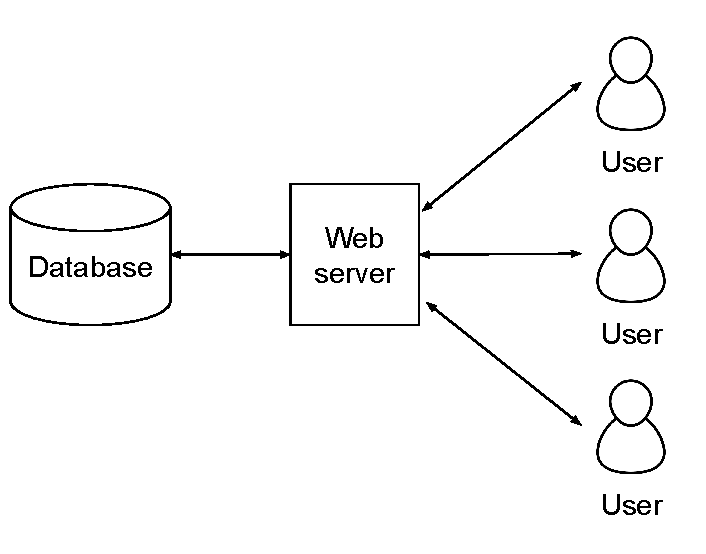
\includegraphics[height=4cm]{./res/img/webserver.pdf}
    \caption{}
    \label{fig:webserver}
  \end{subfigure}
  \hskip 3em
  \begin{subfigure}[m]{.4\textwidth}
    \centering
    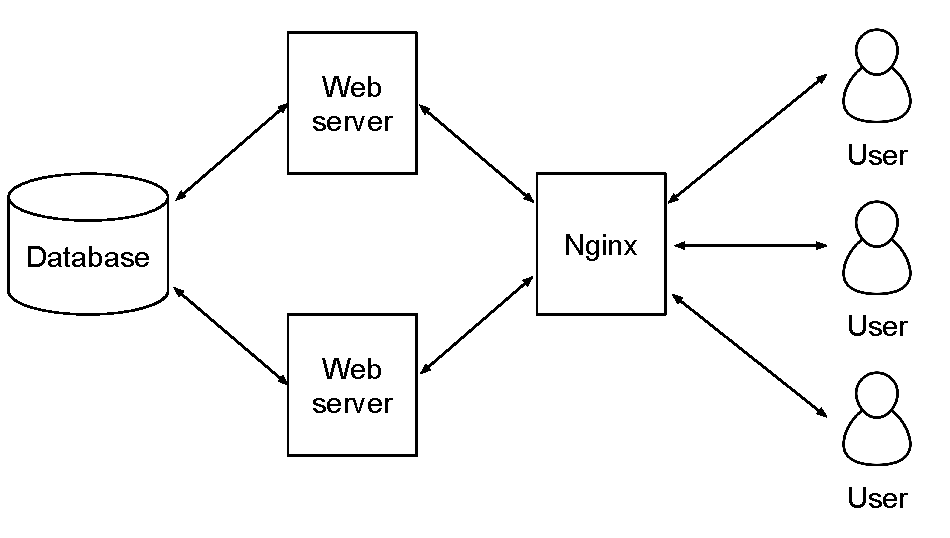
\includegraphics[height=4cm]{./res/img/webserver-nginx.pdf}
    \caption{}
    \label{fig:webserver-nginx}
  \end{subfigure}
  \caption{Web servers without (\protect\subref{fig:webserver}) and with (\protect\subref{fig:webserver-nginx}) load balancer.}
  \label{fig:webserver-scale-x}
\end{figure}

\subsubsection{State}
Let's clarify the concept of \emph{state} in order to better understand the
importance of it for scaling on the x-axis. We said that, in other words, an
application that uses state chooses the next action to be performed evaluating
the current execution condition \cite{bib:art-of-scalability}. This definition
holds for the protocols as well. A common example of stateless protocol is HTTP,
since it does not need to know anything about a previous request having all the
information needed to fulfill the current request. On the contrary, an example
of stateful application is a possible implementation of user session (which can
be done also with a stateless approach), in which a user is authorized to
request some resources only after an authentication request. In this setting,
the result of the authentication could be stored in the server making it
stateful, i.e. some requests are dependent on the authentication request.
Referring at \autoref{fig:webserver-nginx}, in the stateful implementation, the
user sessions could be stored at Web server level. In our example, the only load
balancing method which supports session persistence is \emph{ip-hash} thanks to
its ability to always redirect requests from a client to the same server except
when this server is unavailable or when the client's IP address changes. Indeed,
with \emph{round-robin} and \emph{least-connected} each request is potentially
distributed to a different server making it necessary to write stateless
servers.
% add comparison between this state and the Ethereum state

It should be clear now the role of the \emph{state} scaling on the x-axis. Once
we scale by cloning, we duplicate the data along with the service. If the state
changes, these changes should be reflected on the server which accesses that
same part of the state. This can be not a drawback at first, but it may become
an issue increasing the data size.

\subsubsection{Ethereum current state and proposals}
\label{sec:x-axis-ethereum}
In \autoref{sec:background}, we already pointed out that Ethereum is stateful,
thus making it difficult to scale on the x-axis. As we discussed in
\autoref{sec:network-layer}, the Ethereum implementation uses a peer-to-peer
network in which the nodes are \emph{servent}. Although there are different
clients (e.g. Geth\footnote{\url{https://github.com/ethereum/go-ethereum}},
Parity\footnote{\url{https://github.com/paritytech/parity}},
cpp-ethereum\footnote{\url{https://github.com/ethereum/cpp-ethereum}},
pyethapp\footnote{\url{https://github.com/ethereum/pyethapp}}, ecc.), each one
is compliant with the Ethereum protocols abstracting from the distinct
implementations, so this is not a distinctive characteristic from a functional
perspective. Let's not consider initially the possible different node types
\todo{Here we should discuss the different node types (full, archive, light) or
refer to a section} supposing that it can access the state and that it has its
own copy of it. In \autoref{sec:consensus:algorithm}, we introduced the Ethereum
consensus algorithm and the PoW algorithm which is run by the miners in order to
create the next valid block. The more miners join the network (or improve the
existent), thus incrementing the global hash rate, the more difficult a state
transition become. In \autoref{sec:max-troughput}, we measure the maximal
transaction throughput in a private blockchain\footnote{See \autoref{sec:tests}
for a detailed tests description.}. Incrementing the number of miners in the
network does not increment the transaction throughput, indeed it is almost
negatively affected. This decreasing in performance can be due to a variety of
factors like network overhead, ``unluckiness'' of the miners which affects the
mining difficulty, or perturbation in the performance of the nodes, but it is
not relevant for the purpose of the test. Another significant test we present is
described in \autoref{sec:max-throughput-high-gaslimit}. In this test we set a
gas limit high enough to not restrict the number of transactions which can be
included in a block. The results show a little increment in the transaction
throughput with regards to the previous test, but again the number of miners
does not affect the overall performance. Hence duplicating the miners in the
network does not increment the transaction throughput making the scaling on the
x-axis absent in the current implementation.

Currently, there are no proposals to scale on this direction. The reason
probably lies in the consensus layer. In \autoref{sec:consensus:algorithm}, we
talked about the validation procedure involved in the consensus algorithm.
Everyone validates each block propagated in the network executing all the
transactions and the EVM computations which is in contrast with the concept of
load distribution of the x-axis. Thus, the system is limited by the performance
of the single computer duplicated in the network. In order to scale on this
vector, there should be a balancing of load between the nodes. The proposed
Proof of Stake (see \autoref{sec:pos}) does not scale on the
x-axis, indeed increasing the number of validators doesn't implies a higher
throughput, but maybe a lower ones due to network
overhead\cite{bib:cbc-casper}\todo{Check cite}.

\subsubsection{Proof of Stake}
\label{sec:pos}
Proof of Stake (PoS) is a class of algorithms through which a cryptocurrency
blockchain network achieves distributed consensus. As we have seen in
\autoref{sec:consensus:algorithm}, in PoW the truth is determined by heavy
computation done by the miners. In PoS, there are validators instead of miners
and the consensus depends on the \emph{stake} confirmed by each validator, which
consists in an economic deposit in the network's cryptocurrency (ether in this
case).

\begin{figure}
	\begin{center}
		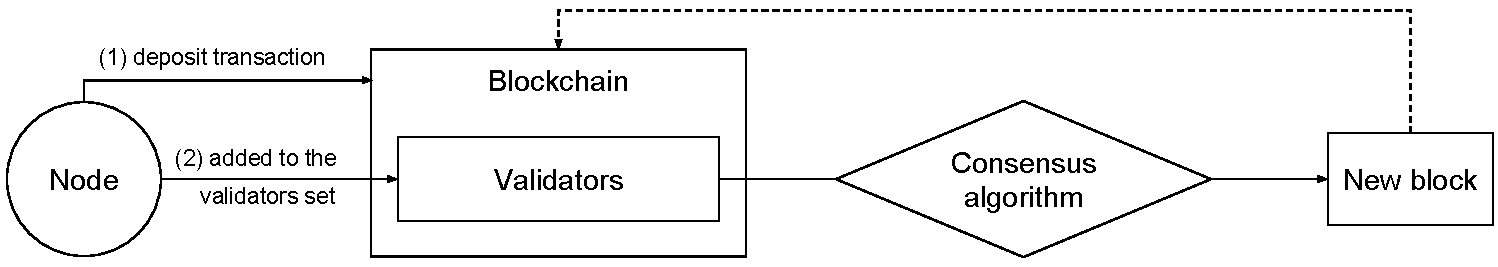
\includegraphics[width=\textwidth]{./res/img/pos.pdf}
	\end{center}
	\caption{Overview of a block creation in the Proof of Stake.}
	\label{fig:pos}
\end{figure}

\autoref{fig:pos} shows a creation of a new block at high level. If a node owns
an amount of the blockchain's base cryptocurrency, it can become a validator
sending a deposit transaction which locks a given value. Once the transaction
has successfully executed, the node becomes one of the validators. The consensus
algorithm determines how a validator is chosen in the set of validators to
\emph{propose} the next block, and then how the validators agree on which block
is canonical. Different type of PoS can be obtained by varying the consensus
algorithm and how the rewards are assigned.


% discutere sui mining pool

% discutere su Infura